\documentclass[twoside]{book}

% Packages required by doxygen
\usepackage{fixltx2e}
\usepackage{calc}
\usepackage{doxygen}
\usepackage[export]{adjustbox} % also loads graphicx
\usepackage{graphicx}
\usepackage[utf8]{inputenc}
\usepackage{makeidx}
\usepackage{multicol}
\usepackage{multirow}
\PassOptionsToPackage{warn}{textcomp}
\usepackage{textcomp}
\usepackage[nointegrals]{wasysym}
\usepackage[table]{xcolor}

% Font selection
\usepackage[T1]{fontenc}
\usepackage[scaled=.90]{helvet}
\usepackage{courier}
\usepackage{amssymb}
\usepackage{sectsty}
\renewcommand{\familydefault}{\sfdefault}
\allsectionsfont{%
  \fontseries{bc}\selectfont%
  \color{darkgray}%
}
\renewcommand{\DoxyLabelFont}{%
  \fontseries{bc}\selectfont%
  \color{darkgray}%
}
\newcommand{\+}{\discretionary{\mbox{\scriptsize$\hookleftarrow$}}{}{}}

% Page & text layout
\usepackage{geometry}
\geometry{%
  a4paper,%
  top=2.5cm,%
  bottom=2.5cm,%
  left=2.5cm,%
  right=2.5cm%
}
\tolerance=750
\hfuzz=15pt
\hbadness=750
\setlength{\emergencystretch}{15pt}
\setlength{\parindent}{0cm}
\setlength{\parskip}{3ex plus 2ex minus 2ex}
\makeatletter
\renewcommand{\paragraph}{%
  \@startsection{paragraph}{4}{0ex}{-1.0ex}{1.0ex}{%
    \normalfont\normalsize\bfseries\SS@parafont%
  }%
}
\renewcommand{\subparagraph}{%
  \@startsection{subparagraph}{5}{0ex}{-1.0ex}{1.0ex}{%
    \normalfont\normalsize\bfseries\SS@subparafont%
  }%
}
\makeatother

% Headers & footers
\usepackage{fancyhdr}
\pagestyle{fancyplain}
\fancyhead[LE]{\fancyplain{}{\bfseries\thepage}}
\fancyhead[CE]{\fancyplain{}{}}
\fancyhead[RE]{\fancyplain{}{\bfseries\leftmark}}
\fancyhead[LO]{\fancyplain{}{\bfseries\rightmark}}
\fancyhead[CO]{\fancyplain{}{}}
\fancyhead[RO]{\fancyplain{}{\bfseries\thepage}}
\fancyfoot[LE]{\fancyplain{}{}}
\fancyfoot[CE]{\fancyplain{}{}}
\fancyfoot[RE]{\fancyplain{}{\bfseries\scriptsize Generated by Doxygen }}
\fancyfoot[LO]{\fancyplain{}{\bfseries\scriptsize Generated by Doxygen }}
\fancyfoot[CO]{\fancyplain{}{}}
\fancyfoot[RO]{\fancyplain{}{}}
\renewcommand{\footrulewidth}{0.4pt}
\renewcommand{\chaptermark}[1]{%
  \markboth{#1}{}%
}
\renewcommand{\sectionmark}[1]{%
  \markright{\thesection\ #1}%
}

% Indices & bibliography
\usepackage{natbib}
\usepackage[titles]{tocloft}
\setcounter{tocdepth}{3}
\setcounter{secnumdepth}{5}
\makeindex

% Hyperlinks (required, but should be loaded last)
\usepackage{ifpdf}
\ifpdf
  \usepackage[pdftex,pagebackref=true]{hyperref}
\else
  \usepackage[ps2pdf,pagebackref=true]{hyperref}
\fi
\hypersetup{%
  colorlinks=true,%
  linkcolor=blue,%
  citecolor=blue,%
  unicode%
}

% Custom commands
\newcommand{\clearemptydoublepage}{%
  \newpage{\pagestyle{empty}\cleardoublepage}%
}

\usepackage{caption}
\captionsetup{labelsep=space,justification=centering,font={bf},singlelinecheck=off,skip=4pt,position=top}

%===== C O N T E N T S =====

\begin{document}

% Titlepage & ToC
\hypersetup{pageanchor=false,
             bookmarksnumbered=true,
             pdfencoding=unicode
            }
\pagenumbering{alph}
\begin{titlepage}
\vspace*{7cm}
\begin{center}%
{\Large M\+O\+H\+I\+D\+\_\+\+Lagr\+Tracer \\[1ex]\large 0.\+01 }\\
\vspace*{1cm}
{\large Generated by Doxygen 1.8.14}\\
\end{center}
\end{titlepage}
\clearemptydoublepage
\pagenumbering{roman}
\tableofcontents
\clearemptydoublepage
\pagenumbering{arabic}
\hypersetup{pageanchor=true}

%--- Begin generated contents ---
\chapter{Modules Index}
\section{Modules List}
Here is a list of all modules with brief descriptions\+:\begin{DoxyCompactList}
\item\contentsline{section}{\mbox{\hyperlink{namespaceabstract__linkedlist__mod}{abstract\+\_\+linkedlist\+\_\+mod}} \\*Module that defines an unlimited polymorphic container list class and related methods. A container is a fundamental entity allowing to build data structures such as lists and arrays. This is an abstract type, so a derived type must be defined for any specific contents that may be required. Those derived types should provide type-\/specific methods that require type-\/guards, such as printing }{\pageref{namespaceabstract__linkedlist__mod}}{}
\item\contentsline{section}{\mbox{\hyperlink{namespaceaot__mod}{aot\+\_\+mod}} \\*Module to hold the Arrays of Tracers class and its methods. This class defines a collection of id, xyz, uvw, .. arrays that allow for easy and efficient manipulation of the Tracer objects. These must be exported into the objects from this class }{\pageref{namespaceaot__mod}}{}
\item\contentsline{section}{\mbox{\hyperlink{namespacebackground__mod}{background\+\_\+mod}} \\*Defines a background class that describes a solution from which to interpolate. A background object contains an arbitrary number of scalar or vectorial fields, in 2, 3 or 4D, indexed to labeled 1D fields of dimensions. The fields are stored in a linked list, enabling trivial iteration }{\pageref{namespacebackground__mod}}{}
\item\contentsline{section}{\mbox{\hyperlink{namespaceblocks__mod}{blocks\+\_\+mod}} \\*Module that defines a block class and related methods. A block is a fundamental type of the model. It contains a sub-\/domain of the simulation bounding box, holding all entities inside that sub-\/domain. It maps to a domain decomposition parallelization strategy, if needed }{\pageref{namespaceblocks__mod}}{}
\item\contentsline{section}{\mbox{\hyperlink{namespaceboundingbox__mod}{boundingbox\+\_\+mod}} \\*Module that defines a simulation Bounding Box }{\pageref{namespaceboundingbox__mod}}{}
\item\contentsline{section}{\mbox{\hyperlink{namespacecommon__modules}{common\+\_\+modules}} \\*Module to hold all of the commonly used base modules }{\pageref{namespacecommon__modules}}{}
\item\contentsline{section}{\mbox{\hyperlink{namespacecontainer__mod}{container\+\_\+mod}} \\*Module that defines an unlimited polymorphic container class and related methods. A container is a fundamental entity allowing to build data structures such as lists and arrays }{\pageref{namespacecontainer__mod}}{}
\item\contentsline{section}{\mbox{\hyperlink{namespaceemitter__mod}{emitter\+\_\+mod}} \\*Module that defines an emitter class and related methods. This module is responsible for building a potential tracer list based on the availble sources and calling their initializers }{\pageref{namespaceemitter__mod}}{}
\item\contentsline{section}{\mbox{\hyperlink{namespacefield__types__mod}{field\+\_\+types\+\_\+mod}} \\*Defines classes for \textquotesingle{}fields\textquotesingle{}\+: 1, 2, 3 and 4D labeled data. Valid for both scalar and vectorial (real) data. Defines a generic wrapper for these classes, that abstracts the user from having to choose their data dimensionality or type to create a field }{\pageref{namespacefield__types__mod}}{}
\item\contentsline{section}{\mbox{\hyperlink{namespacegeometry__mod}{geometry\+\_\+mod}} \\*Module that defines geometry classes and related methods }{\pageref{namespacegeometry__mod}}{}
\item\contentsline{section}{\mbox{\hyperlink{namespaceinterpolator__mod}{interpolator\+\_\+mod}} \\*Defines an Interpolator class }{\pageref{namespaceinterpolator__mod}}{}
\item\contentsline{section}{\mbox{\hyperlink{namespacelink__mod}{link\+\_\+mod}} \\*Module that defines a link based on an unlimited polymorphic container class }{\pageref{namespacelink__mod}}{}
\item\contentsline{section}{\mbox{\hyperlink{namespacesimulation__about__mod}{simulation\+\_\+about\+\_\+mod}} \\*Module to print version, licence, preambles }{\pageref{namespacesimulation__about__mod}}{}
\item\contentsline{section}{\mbox{\hyperlink{namespacesimulation__globals__mod}{simulation\+\_\+globals\+\_\+mod}} \\*Module to hold the simulation global parameter classes and their methods }{\pageref{namespacesimulation__globals__mod}}{}
\item\contentsline{section}{\mbox{\hyperlink{namespacesimulation__initialize__mod}{simulation\+\_\+initialize\+\_\+mod}} \\*Module with the simulation initialization related definitions and methods. Has one public access routine that is incharge of building the simulation space from input files }{\pageref{namespacesimulation__initialize__mod}}{}
\item\contentsline{section}{\mbox{\hyperlink{namespacesimulation__logger__mod}{simulation\+\_\+logger\+\_\+mod}} \\*Module to hold all the simulation logger related definitions and methods }{\pageref{namespacesimulation__logger__mod}}{}
\item\contentsline{section}{\mbox{\hyperlink{namespacesimulation__memory__mod}{simulation\+\_\+memory\+\_\+mod}} \\*Module to hold the simulation memory managment class and its methods }{\pageref{namespacesimulation__memory__mod}}{}
\item\contentsline{section}{\mbox{\hyperlink{namespacesimulation__mod}{simulation\+\_\+mod}} \\*Module to hold the simulation class and its methods. This is the only class that is exposed to an external program, as it encapsulates every other class and method }{\pageref{namespacesimulation__mod}}{}
\item\contentsline{section}{\mbox{\hyperlink{namespacesimulation__output__streamer__mod}{simulation\+\_\+output\+\_\+streamer\+\_\+mod}} \\*Defines a output file writer class with an object exposable to the Simulation This class is in charge of selectig the correct writter for the selected output file format }{\pageref{namespacesimulation__output__streamer__mod}}{}
\item\contentsline{section}{\mbox{\hyperlink{namespacesimulation__precision__mod}{simulation\+\_\+precision\+\_\+mod}} \\*Module to control the precision of the variables trough the project }{\pageref{namespacesimulation__precision__mod}}{}
\item\contentsline{section}{\mbox{\hyperlink{namespacesolver__mod}{solver\+\_\+mod}} \\*Defines an Solver class. This class invokes the different available integration algorithms as methods, and these invoke the necessary interpolation objects }{\pageref{namespacesolver__mod}}{}
\item\contentsline{section}{\mbox{\hyperlink{namespacesources__list__mod}{sources\+\_\+list\+\_\+mod}} \\*Module to hold the Sources linked list class and its methods. This class defines a double linked list to store any variable type, but with specific methods with type guards for Source objects. The class allows for insertion, deletion and iteration of the desired contents }{\pageref{namespacesources__list__mod}}{}
\item\contentsline{section}{\mbox{\hyperlink{namespacesources__mod}{sources\+\_\+mod}} \\*Module that defines a source class and related methods }{\pageref{namespacesources__mod}}{}
\item\contentsline{section}{\mbox{\hyperlink{namespacetracer__base__mod}{tracer\+\_\+base\+\_\+mod}} \\*Module that defines a pure Lagrangian tracer class and related methods }{\pageref{namespacetracer__base__mod}}{}
\item\contentsline{section}{\mbox{\hyperlink{namespacetracer__list__mod}{tracer\+\_\+list\+\_\+mod}} \\*Module to hold the tracer linked list class and its methods. This class defines a double linked list to store any variable type, but with specific methods with type guards for Tracer objects. The class allows for insertion, deletion and iteration of the desired contents }{\pageref{namespacetracer__list__mod}}{}
\item\contentsline{section}{\mbox{\hyperlink{namespacetracer__paper__mod}{tracer\+\_\+paper\+\_\+mod}} \\*Module that defines a Lagrangian tracer class for paper modelling and related methods. The type is defined as a derived type from the pule Lagrangian tracer, and hence inherits all of it\textquotesingle{}s data and methods }{\pageref{namespacetracer__paper__mod}}{}
\item\contentsline{section}{\mbox{\hyperlink{namespacetracer__plastic__mod}{tracer\+\_\+plastic\+\_\+mod}} \\*Module that defines a Lagrangian tracer class for plastic modelling and related methods. The type is defined as a derived type from the pule Lagrangian tracer, and hence inherits all of it\textquotesingle{}s data and methods }{\pageref{namespacetracer__plastic__mod}}{}
\item\contentsline{section}{\mbox{\hyperlink{namespacetracers__mod}{tracers\+\_\+mod}} \\*Module to hold and \textquotesingle{}wrap\textquotesingle{} all the tracer respective modules }{\pageref{namespacetracers__mod}}{}
\item\contentsline{section}{\mbox{\hyperlink{namespaceutilities__mod}{utilities\+\_\+mod}} \\*Module that provides useful back-\/end routines }{\pageref{namespaceutilities__mod}}{}
\item\contentsline{section}{\mbox{\hyperlink{namespacevtkwritter__mod}{vtkwritter\+\_\+mod}} \\*Defines a vtk writer class with an object exposable to the Output streamer. Writes files in .xml vtk, both in serial and parallel model. Uses an unstructured mesh format specifier to store any type of data, both meshes and Tracers. Supports scalar and vectorial data }{\pageref{namespacevtkwritter__mod}}{}
\item\contentsline{section}{\mbox{\hyperlink{namespacexmlparser__mod}{xmlparser\+\_\+mod}} \\*Module with the simulation xml parsing class and methods, Encapsulates the F\+O\+X\+\_\+dom library }{\pageref{namespacexmlparser__mod}}{}
\end{DoxyCompactList}

\chapter{Data Type Index}
\section{Data Types List}
Here are the data types with brief descriptions\+:\begin{DoxyCompactList}
\item\contentsline{section}{\mbox{\hyperlink{interfacebackground__mod_1_1background}{background\+\_\+mod\+::background}} }{\pageref{interfacebackground__mod_1_1background}}{}
\item\contentsline{section}{\mbox{\hyperlink{structbackground__mod_1_1background__class}{background\+\_\+mod\+::background\+\_\+class}} }{\pageref{structbackground__mod_1_1background__class}}{}
\item\contentsline{section}{\mbox{\hyperlink{structblocks__mod_1_1block__class}{blocks\+\_\+mod\+::block\+\_\+class}} }{\pageref{structblocks__mod_1_1block__class}}{}
\item\contentsline{section}{\mbox{\hyperlink{structboundingbox__mod_1_1boundingbox__class}{boundingbox\+\_\+mod\+::boundingbox\+\_\+class}} }{\pageref{structboundingbox__mod_1_1boundingbox__class}}{}
\item\contentsline{section}{\mbox{\hyperlink{structgeometry__mod_1_1box}{geometry\+\_\+mod\+::box}} \\*Type -\/ point class }{\pageref{structgeometry__mod_1_1box}}{}
\item\contentsline{section}{\mbox{\hyperlink{structsimulationglobals__mod_1_1constants__t}{simulationglobals\+\_\+mod\+::constants\+\_\+t}} \\*Case Constants class }{\pageref{structsimulationglobals__mod_1_1constants__t}}{}
\item\contentsline{section}{\mbox{\hyperlink{structcontainer__mod_1_1container}{container\+\_\+mod\+::container}} }{\pageref{structcontainer__mod_1_1container}}{}
\item\contentsline{section}{\mbox{\hyperlink{structcsvparser__mod_1_1csvparser__class}{csvparser\+\_\+mod\+::csvparser\+\_\+class}} }{\pageref{structcsvparser__mod_1_1csvparser__class}}{}
\item\contentsline{section}{\mbox{\hyperlink{structnetcdfparser__mod_1_1dim__t}{netcdfparser\+\_\+mod\+::dim\+\_\+t}} }{\pageref{structnetcdfparser__mod_1_1dim__t}}{}
\item\contentsline{section}{\mbox{\hyperlink{structemitter__mod_1_1emitter__class}{emitter\+\_\+mod\+::emitter\+\_\+class}} }{\pageref{structemitter__mod_1_1emitter__class}}{}
\item\contentsline{section}{\mbox{\hyperlink{structfieldtypes__mod_1_1field__class}{fieldtypes\+\_\+mod\+::field\+\_\+class}} }{\pageref{structfieldtypes__mod_1_1field__class}}{}
\item\contentsline{section}{\mbox{\hyperlink{structbackground__mod_1_1fieldslist__class}{background\+\_\+mod\+::fieldslist\+\_\+class}} }{\pageref{structbackground__mod_1_1fieldslist__class}}{}
\item\contentsline{section}{\mbox{\hyperlink{structsimulationglobals__mod_1_1filenames__t}{simulationglobals\+\_\+mod\+::filenames\+\_\+t}} \\*File names class }{\pageref{structsimulationglobals__mod_1_1filenames__t}}{}
\item\contentsline{section}{\mbox{\hyperlink{structfieldtypes__mod_1_1generic__field__class}{fieldtypes\+\_\+mod\+::generic\+\_\+field\+\_\+class}} \\*Generic field class. This works as a wrapper for a generic initialization routine }{\pageref{structfieldtypes__mod_1_1generic__field__class}}{}
\item\contentsline{section}{\mbox{\hyperlink{structgeometry__mod_1_1geometry__class}{geometry\+\_\+mod\+::geometry\+\_\+class}} }{\pageref{structgeometry__mod_1_1geometry__class}}{}
\item\contentsline{section}{\mbox{\hyperlink{structsimulationglobals__mod_1_1globals__class}{simulationglobals\+\_\+mod\+::globals\+\_\+class}} \\*Globals class -\/ This is a container for every global variable on the simulation }{\pageref{structsimulationglobals__mod_1_1globals__class}}{}
\item\contentsline{section}{\mbox{\hyperlink{structsimulationinputstreamer__mod_1_1input__streamer__class}{simulationinputstreamer\+\_\+mod\+::input\+\_\+streamer\+\_\+class}} \\*Input Streamer class }{\pageref{structsimulationinputstreamer__mod_1_1input__streamer__class}}{}
\item\contentsline{section}{\mbox{\hyperlink{structsimulationinputstreamer__mod_1_1inputfilemodel__class}{simulationinputstreamer\+\_\+mod\+::inputfilemodel\+\_\+class}} }{\pageref{structsimulationinputstreamer__mod_1_1inputfilemodel__class}}{}
\item\contentsline{section}{\mbox{\hyperlink{structinterpolator__mod_1_1interpolator__class}{interpolator\+\_\+mod\+::interpolator\+\_\+class}} }{\pageref{structinterpolator__mod_1_1interpolator__class}}{}
\item\contentsline{section}{\mbox{\hyperlink{structkernel__mod_1_1kernel__class}{kernel\+\_\+mod\+::kernel\+\_\+class}} }{\pageref{structkernel__mod_1_1kernel__class}}{}
\item\contentsline{section}{\mbox{\hyperlink{structgeometry__mod_1_1line}{geometry\+\_\+mod\+::line}} \\*Type -\/ line class }{\pageref{structgeometry__mod_1_1line}}{}
\item\contentsline{section}{\mbox{\hyperlink{structlink__mod_1_1link}{link\+\_\+mod\+::link}} }{\pageref{structlink__mod_1_1link}}{}
\item\contentsline{section}{\mbox{\hyperlink{structabstract__linkedlist__mod_1_1linkedlist}{abstract\+\_\+linkedlist\+\_\+mod\+::linkedlist}} }{\pageref{structabstract__linkedlist__mod_1_1linkedlist}}{}
\item\contentsline{section}{\mbox{\hyperlink{structsimulationlogger__mod_1_1logger__class}{simulationlogger\+\_\+mod\+::logger\+\_\+class}} }{\pageref{structsimulationlogger__mod_1_1logger__class}}{}
\item\contentsline{section}{\mbox{\hyperlink{structsimulationglobals__mod_1_1maskvals__t}{simulationglobals\+\_\+mod\+::maskvals\+\_\+t}} }{\pageref{structsimulationglobals__mod_1_1maskvals__t}}{}
\item\contentsline{section}{\mbox{\hyperlink{structsimulationmemory__mod_1_1memory__t}{simulationmemory\+\_\+mod\+::memory\+\_\+t}} }{\pageref{structsimulationmemory__mod_1_1memory__t}}{}
\item\contentsline{section}{\mbox{\hyperlink{structnetcdfparser__mod_1_1ncfile__class}{netcdfparser\+\_\+mod\+::ncfile\+\_\+class}} \\*A class that models a netcdf file }{\pageref{structnetcdfparser__mod_1_1ncfile__class}}{}
\item\contentsline{section}{\mbox{\hyperlink{structsimulationoutputstreamer__mod_1_1output__streamer__class}{simulationoutputstreamer\+\_\+mod\+::output\+\_\+streamer\+\_\+class}} }{\pageref{structsimulationoutputstreamer__mod_1_1output__streamer__class}}{}
\item\contentsline{section}{\mbox{\hyperlink{structtracerpaper__mod_1_1paper__class}{tracerpaper\+\_\+mod\+::paper\+\_\+class}} \\*Type -\/ The plastic material Lagrangian tracer class }{\pageref{structtracerpaper__mod_1_1paper__class}}{}
\item\contentsline{section}{\mbox{\hyperlink{structtracerpaper__mod_1_1paper__par__class}{tracerpaper\+\_\+mod\+::paper\+\_\+par\+\_\+class}} }{\pageref{structtracerpaper__mod_1_1paper__par__class}}{}
\item\contentsline{section}{\mbox{\hyperlink{structtracerpaper__mod_1_1paper__state__class}{tracerpaper\+\_\+mod\+::paper\+\_\+state\+\_\+class}} \\*Type -\/ State variables of a tracer object representing a paper material }{\pageref{structtracerpaper__mod_1_1paper__state__class}}{}
\item\contentsline{section}{\mbox{\hyperlink{interfacetracerpaper__mod_1_1papertracer}{tracerpaper\+\_\+mod\+::papertracer}} }{\pageref{interfacetracerpaper__mod_1_1papertracer}}{}
\item\contentsline{section}{\mbox{\hyperlink{structsimulationparallel__omp__mod_1_1parallel__omp__class}{simulationparallel\+\_\+omp\+\_\+mod\+::parallel\+\_\+omp\+\_\+class}} }{\pageref{structsimulationparallel__omp__mod_1_1parallel__omp__class}}{}
\item\contentsline{section}{\mbox{\hyperlink{structsimulationglobals__mod_1_1parameters__t}{simulationglobals\+\_\+mod\+::parameters\+\_\+t}} }{\pageref{structsimulationglobals__mod_1_1parameters__t}}{}
\item\contentsline{section}{\mbox{\hyperlink{structtracerplastic__mod_1_1plastic__class}{tracerplastic\+\_\+mod\+::plastic\+\_\+class}} \\*Type -\/ The plastic material Lagrangian tracer class }{\pageref{structtracerplastic__mod_1_1plastic__class}}{}
\item\contentsline{section}{\mbox{\hyperlink{structtracerplastic__mod_1_1plastic__par__class}{tracerplastic\+\_\+mod\+::plastic\+\_\+par\+\_\+class}} }{\pageref{structtracerplastic__mod_1_1plastic__par__class}}{}
\item\contentsline{section}{\mbox{\hyperlink{structtracerplastic__mod_1_1plastic__state__class}{tracerplastic\+\_\+mod\+::plastic\+\_\+state\+\_\+class}} \\*Type -\/ State variables of a tracer object representing a plastic material }{\pageref{structtracerplastic__mod_1_1plastic__state__class}}{}
\item\contentsline{section}{\mbox{\hyperlink{interfacetracerplastic__mod_1_1plastictracer}{tracerplastic\+\_\+mod\+::plastictracer}} }{\pageref{interfacetracerplastic__mod_1_1plastictracer}}{}
\item\contentsline{section}{\mbox{\hyperlink{structgeometry__mod_1_1point}{geometry\+\_\+mod\+::point}} \\*Type -\/ point class }{\pageref{structgeometry__mod_1_1point}}{}
\item\contentsline{section}{\mbox{\hyperlink{structfieldtypes__mod_1_1scalar1d__field__class}{fieldtypes\+\_\+mod\+::scalar1d\+\_\+field\+\_\+class}} \\*1D scalar field class }{\pageref{structfieldtypes__mod_1_1scalar1d__field__class}}{}
\item\contentsline{section}{\mbox{\hyperlink{structfieldtypes__mod_1_1scalar2d__field__class}{fieldtypes\+\_\+mod\+::scalar2d\+\_\+field\+\_\+class}} \\*2D scalar field class }{\pageref{structfieldtypes__mod_1_1scalar2d__field__class}}{}
\item\contentsline{section}{\mbox{\hyperlink{structfieldtypes__mod_1_1scalar3d__field__class}{fieldtypes\+\_\+mod\+::scalar3d\+\_\+field\+\_\+class}} \\*3D scalar field class }{\pageref{structfieldtypes__mod_1_1scalar3d__field__class}}{}
\item\contentsline{section}{\mbox{\hyperlink{structfieldtypes__mod_1_1scalar4d__field__class}{fieldtypes\+\_\+mod\+::scalar4d\+\_\+field\+\_\+class}} \\*4D scalar field class }{\pageref{structfieldtypes__mod_1_1scalar4d__field__class}}{}
\item\contentsline{section}{\mbox{\hyperlink{structfieldtypes__mod_1_1scalar__field__class}{fieldtypes\+\_\+mod\+::scalar\+\_\+field\+\_\+class}} \\*Scalar field class }{\pageref{structfieldtypes__mod_1_1scalar__field__class}}{}
\item\contentsline{section}{\mbox{\hyperlink{structgeometry__mod_1_1shape}{geometry\+\_\+mod\+::shape}} \\*Type -\/ extendable shape class }{\pageref{structgeometry__mod_1_1shape}}{}
\item\contentsline{section}{\mbox{\hyperlink{structsimulationglobals__mod_1_1sim__t}{simulationglobals\+\_\+mod\+::sim\+\_\+t}} \\*Simulation related counters and others }{\pageref{structsimulationglobals__mod_1_1sim__t}}{}
\item\contentsline{section}{\mbox{\hyperlink{structsimulationglobals__mod_1_1sim__time__t}{simulationglobals\+\_\+mod\+::sim\+\_\+time\+\_\+t}} }{\pageref{structsimulationglobals__mod_1_1sim__time__t}}{}
\item\contentsline{section}{\mbox{\hyperlink{structsimulationglobals__mod_1_1simdefs__t}{simulationglobals\+\_\+mod\+::simdefs\+\_\+t}} \\*Simulation definitions class }{\pageref{structsimulationglobals__mod_1_1simdefs__t}}{}
\item\contentsline{section}{\mbox{\hyperlink{structsimulation__mod_1_1simulation__class}{simulation\+\_\+mod\+::simulation\+\_\+class}} }{\pageref{structsimulation__mod_1_1simulation__class}}{}
\item\contentsline{section}{\mbox{\hyperlink{structsolver__mod_1_1solver__class}{solver\+\_\+mod\+::solver\+\_\+class}} }{\pageref{structsolver__mod_1_1solver__class}}{}
\item\contentsline{section}{\mbox{\hyperlink{structsources__mod_1_1source__class}{sources\+\_\+mod\+::source\+\_\+class}} \\*Type -\/ The source class }{\pageref{structsources__mod_1_1source__class}}{}
\item\contentsline{section}{\mbox{\hyperlink{structsources__mod_1_1source__group__class}{sources\+\_\+mod\+::source\+\_\+group\+\_\+class}} }{\pageref{structsources__mod_1_1source__group__class}}{}
\item\contentsline{section}{\mbox{\hyperlink{structsources__mod_1_1source__par}{sources\+\_\+mod\+::source\+\_\+par}} }{\pageref{structsources__mod_1_1source__par}}{}
\item\contentsline{section}{\mbox{\hyperlink{structsources__mod_1_1source__prop}{sources\+\_\+mod\+::source\+\_\+prop}} \\*Type -\/ material properties of a source object }{\pageref{structsources__mod_1_1source__prop}}{}
\item\contentsline{section}{\mbox{\hyperlink{structsources__mod_1_1source__state}{sources\+\_\+mod\+::source\+\_\+state}} \\*Type -\/ state variables of a source object }{\pageref{structsources__mod_1_1source__state}}{}
\item\contentsline{section}{\mbox{\hyperlink{structsources__mod_1_1source__stats}{sources\+\_\+mod\+::source\+\_\+stats}} \\*Type -\/ statistical variables of a source object }{\pageref{structsources__mod_1_1source__stats}}{}
\item\contentsline{section}{\mbox{\hyperlink{structsources__mod_1_1source__stencil}{sources\+\_\+mod\+::source\+\_\+stencil}} \\*Type -\/ holder for the tracer creation stencil of the source }{\pageref{structsources__mod_1_1source__stencil}}{}
\item\contentsline{section}{\mbox{\hyperlink{structsourceslist__mod_1_1sourcelist__class}{sourceslist\+\_\+mod\+::sourcelist\+\_\+class}} }{\pageref{structsourceslist__mod_1_1sourcelist__class}}{}
\item\contentsline{section}{\mbox{\hyperlink{structgeometry__mod_1_1sphere}{geometry\+\_\+mod\+::sphere}} \\*Type -\/ sphere class }{\pageref{structgeometry__mod_1_1sphere}}{}
\item\contentsline{section}{\mbox{\hyperlink{structsimulationglobals__mod_1_1src__parm__t}{simulationglobals\+\_\+mod\+::src\+\_\+parm\+\_\+t}} \\*Lists for Source parameters }{\pageref{structsimulationglobals__mod_1_1src__parm__t}}{}
\item\contentsline{section}{\mbox{\hyperlink{structstatevector__mod_1_1statevector__class}{statevector\+\_\+mod\+::statevector\+\_\+class}} }{\pageref{structstatevector__mod_1_1statevector__class}}{}
\item\contentsline{section}{\mbox{\hyperlink{structsimulationglobals__mod_1_1stringlist__class}{simulationglobals\+\_\+mod\+::stringlist\+\_\+class}} }{\pageref{structsimulationglobals__mod_1_1stringlist__class}}{}
\item\contentsline{section}{\mbox{\hyperlink{structsimulationtestmaker__mod_1_1testmaker__class}{simulationtestmaker\+\_\+mod\+::testmaker\+\_\+class}} }{\pageref{structsimulationtestmaker__mod_1_1testmaker__class}}{}
\item\contentsline{section}{\mbox{\hyperlink{structsimulationtimer__mod_1_1timer__class}{simulationtimer\+\_\+mod\+::timer\+\_\+class}} }{\pageref{structsimulationtimer__mod_1_1timer__class}}{}
\item\contentsline{section}{\mbox{\hyperlink{interfacetracerbase__mod_1_1tracer}{tracerbase\+\_\+mod\+::tracer}} }{\pageref{interfacetracerbase__mod_1_1tracer}}{}
\item\contentsline{section}{\mbox{\hyperlink{structtracerbase__mod_1_1tracer__class}{tracerbase\+\_\+mod\+::tracer\+\_\+class}} \\*Type -\/ The pure Lagrangian tracer class }{\pageref{structtracerbase__mod_1_1tracer__class}}{}
\item\contentsline{section}{\mbox{\hyperlink{structtracerbase__mod_1_1tracer__par__class}{tracerbase\+\_\+mod\+::tracer\+\_\+par\+\_\+class}} }{\pageref{structtracerbase__mod_1_1tracer__par__class}}{}
\item\contentsline{section}{\mbox{\hyperlink{structtracerbase__mod_1_1tracer__state__class}{tracerbase\+\_\+mod\+::tracer\+\_\+state\+\_\+class}} \\*Type -\/ state variables of a pure Lagrangian tracer object }{\pageref{structtracerbase__mod_1_1tracer__state__class}}{}
\item\contentsline{section}{\mbox{\hyperlink{structtracerlist__mod_1_1tracerlist__class}{tracerlist\+\_\+mod\+::tracerlist\+\_\+class}} }{\pageref{structtracerlist__mod_1_1tracerlist__class}}{}
\item\contentsline{section}{\mbox{\hyperlink{structsimulationglobals__mod_1_1tracertypes__t}{simulationglobals\+\_\+mod\+::tracertypes\+\_\+t}} }{\pageref{structsimulationglobals__mod_1_1tracertypes__t}}{}
\item\contentsline{section}{\mbox{\hyperlink{structstatevector__mod_1_1trcptr__class}{statevector\+\_\+mod\+::trcptr\+\_\+class}} }{\pageref{structstatevector__mod_1_1trcptr__class}}{}
\item\contentsline{section}{\mbox{\hyperlink{structtraceruser__mod_1_1user__par__class}{traceruser\+\_\+mod\+::user\+\_\+par\+\_\+class}} }{\pageref{structtraceruser__mod_1_1user__par__class}}{}
\item\contentsline{section}{\mbox{\hyperlink{structtraceruser__mod_1_1user__state__class}{traceruser\+\_\+mod\+::user\+\_\+state\+\_\+class}} \\*Type -\/ State variables of a tracer object representing a user defined type }{\pageref{structtraceruser__mod_1_1user__state__class}}{}
\item\contentsline{section}{\mbox{\hyperlink{interfacetraceruser__mod_1_1usertracer}{traceruser\+\_\+mod\+::usertracer}} }{\pageref{interfacetraceruser__mod_1_1usertracer}}{}
\item\contentsline{section}{\mbox{\hyperlink{structtraceruser__mod_1_1usertracer__class}{traceruser\+\_\+mod\+::usertracer\+\_\+class}} \\*Type -\/ The user-\/defined Lagrangian tracer class }{\pageref{structtraceruser__mod_1_1usertracer__class}}{}
\item\contentsline{section}{\mbox{\hyperlink{structutilities__mod_1_1utils__class}{utilities\+\_\+mod\+::utils\+\_\+class}} }{\pageref{structutilities__mod_1_1utils__class}}{}
\item\contentsline{section}{\mbox{\hyperlink{structsimulationglobals__mod_1_1var__names__t}{simulationglobals\+\_\+mod\+::var\+\_\+names\+\_\+t}} }{\pageref{structsimulationglobals__mod_1_1var__names__t}}{}
\item\contentsline{section}{\mbox{\hyperlink{structnetcdfparser__mod_1_1var__t}{netcdfparser\+\_\+mod\+::var\+\_\+t}} }{\pageref{structnetcdfparser__mod_1_1var__t}}{}
\item\contentsline{section}{\mbox{\hyperlink{structfieldtypes__mod_1_1vectorial2d__field__class}{fieldtypes\+\_\+mod\+::vectorial2d\+\_\+field\+\_\+class}} \\*2D vectorial field class }{\pageref{structfieldtypes__mod_1_1vectorial2d__field__class}}{}
\item\contentsline{section}{\mbox{\hyperlink{structfieldtypes__mod_1_1vectorial3d__field__class}{fieldtypes\+\_\+mod\+::vectorial3d\+\_\+field\+\_\+class}} \\*3D vectorial field class }{\pageref{structfieldtypes__mod_1_1vectorial3d__field__class}}{}
\item\contentsline{section}{\mbox{\hyperlink{structfieldtypes__mod_1_1vectorial4d__field__class}{fieldtypes\+\_\+mod\+::vectorial4d\+\_\+field\+\_\+class}} \\*4D vectorial field class }{\pageref{structfieldtypes__mod_1_1vectorial4d__field__class}}{}
\item\contentsline{section}{\mbox{\hyperlink{structfieldtypes__mod_1_1vectorial__field__class}{fieldtypes\+\_\+mod\+::vectorial\+\_\+field\+\_\+class}} \\*Vectorial field class }{\pageref{structfieldtypes__mod_1_1vectorial__field__class}}{}
\item\contentsline{section}{\mbox{\hyperlink{structvtkwritter__mod_1_1vtkwritter__class}{vtkwritter\+\_\+mod\+::vtkwritter\+\_\+class}} }{\pageref{structvtkwritter__mod_1_1vtkwritter__class}}{}
\item\contentsline{section}{\mbox{\hyperlink{structxmlparser__mod_1_1xmlparser__class}{xmlparser\+\_\+mod\+::xmlparser\+\_\+class}} }{\pageref{structxmlparser__mod_1_1xmlparser__class}}{}
\end{DoxyCompactList}

\chapter{Module Documentation}
\hypertarget{namespacetracer}{}\section{tracer Module Reference}
\label{namespacetracer}\index{tracer@{tracer}}


Module to hold and wrap all the tracer respective modules. Defines a pure Lagrangian tracer class. This is intended to serve as the base class for every type of tracer class needed, that should be ~\newline
 built as derived of this class, with the necessary modifiers to model the desired behaviour. Basic tracer data (parameters, variables) are implemented. Tracer methods such as I/O, integration and interpolation routines are implemented.  




\subsection{Detailed Description}
Module to hold and wrap all the tracer respective modules. Defines a pure Lagrangian tracer class. This is intended to serve as the base class for every type of tracer class needed, that should be ~\newline
 built as derived of this class, with the necessary modifiers to model the desired behaviour. Basic tracer data (parameters, variables) are implemented. Tracer methods such as I/O, integration and interpolation routines are implemented. 

\begin{DoxyAuthor}{Author}
Ricardo Birjukovs Canelas 
\end{DoxyAuthor}

\hypertarget{namespacetracer2d}{}\section{tracer2d Module Reference}
\label{namespacetracer2d}\index{tracer2d@{tracer2d}}


Module that defines a pure Lagrangian 2D tracer class and related methods, as a subset of the tracer3D module.  


\subsection*{Functions/\+Subroutines}
\begin{DoxyCompactItemize}
\item 
subroutine \mbox{\hyperlink{namespacetracer2d_abebf96ac23ed37832000c68fea45f584}{tracer2d\+\_\+init}} (trc, filename, time, x, is\+\_\+sigma)
\begin{DoxyCompactList}\small\item\em Birjukovs Canelas -\/ M\+A\+R\+E\+T\+EC Routine Author Name and Affiliation. \end{DoxyCompactList}\end{DoxyCompactItemize}


\subsection{Detailed Description}
Module that defines a pure Lagrangian 2D tracer class and related methods, as a subset of the tracer3D module. 

\begin{DoxyAuthor}{Author}
Ricardo Birjukovs Canelas 
\end{DoxyAuthor}


\subsection{Function/\+Subroutine Documentation}
\mbox{\Hypertarget{namespacetracer2d_abebf96ac23ed37832000c68fea45f584}\label{namespacetracer2d_abebf96ac23ed37832000c68fea45f584}} 
\index{tracer2d@{tracer2d}!tracer2d\+\_\+init@{tracer2d\+\_\+init}}
\index{tracer2d\+\_\+init@{tracer2d\+\_\+init}!tracer2d@{tracer2d}}
\subsubsection{\texorpdfstring{tracer2d\+\_\+init()}{tracer2d\_init()}}
{\footnotesize\ttfamily subroutine tracer2d\+::tracer2d\+\_\+init (\begin{DoxyParamCaption}\item[{type(tracer\+\_\+class), intent(out)}]{trc,  }\item[{character(len=$\ast$), intent(in)}]{filename,  }\item[{real(prec\+\_\+time)}]{time,  }\item[{real(prec), dimension(\+:), intent(in)}]{x,  }\item[{logical, intent(in)}]{is\+\_\+sigma }\end{DoxyParamCaption})}



Birjukovs Canelas -\/ M\+A\+R\+E\+T\+EC Routine Author Name and Affiliation. 

Brief description of routine.

2D Tracer inititialization routine -\/ Generates a tracer collection and initializes their variables 
\begin{DoxyParams}[1]{Parameters}
\mbox{\tt out}  & {\em trc} & ~\newline
\\
\hline
\mbox{\tt in}  & {\em filename} & \\
\hline
\end{DoxyParams}

\hypertarget{namespacetracer3d}{}\section{tracer3d Module Reference}
\label{namespacetracer3d}\index{tracer3d@{tracer3d}}


Module that defines a pure Lagrangian tracer class and related methods.  


\subsection*{Functions/\+Subroutines}
\begin{DoxyCompactItemize}
\item 
subroutine, public \mbox{\hyperlink{namespacetracer3d_a42aa514ae0b5c46c797ddaaa48c49991}{tracer\+\_\+init}} (trc, id, time, x, y, z)
\begin{DoxyCompactList}\small\item\em Birjukovs Canelas -\/ M\+A\+R\+E\+T\+EC \end{DoxyCompactList}\end{DoxyCompactItemize}


\subsection{Detailed Description}
Module that defines a pure Lagrangian tracer class and related methods. 

\begin{DoxyAuthor}{Author}
Ricardo Birjukovs Canelas 
\end{DoxyAuthor}


\subsection{Function/\+Subroutine Documentation}
\mbox{\Hypertarget{namespacetracer3d_a42aa514ae0b5c46c797ddaaa48c49991}\label{namespacetracer3d_a42aa514ae0b5c46c797ddaaa48c49991}} 
\index{tracer3d@{tracer3d}!tracer\+\_\+init@{tracer\+\_\+init}}
\index{tracer\+\_\+init@{tracer\+\_\+init}!tracer3d@{tracer3d}}
\subsubsection{\texorpdfstring{tracer\+\_\+init()}{tracer\_init()}}
{\footnotesize\ttfamily subroutine, public tracer3d\+::tracer\+\_\+init (\begin{DoxyParamCaption}\item[{type(tracer\+\_\+class), intent(out)}]{trc,  }\item[{integer, intent(in)}]{id,  }\item[{real(prec\+\_\+time), intent(in)}]{time,  }\item[{real(prec), intent(in)}]{x,  }\item[{real(prec), intent(in)}]{y,  }\item[{real(prec), intent(in)}]{z }\end{DoxyParamCaption})}



Birjukovs Canelas -\/ M\+A\+R\+E\+T\+EC 

Tracer inititialization routine -\/ Generates a tracer and initializes its variables 
\begin{DoxyParams}[1]{Parameters}
\mbox{\tt out}  & {\em trc} & ~\newline
\\
\hline
\mbox{\tt in}  & {\em filename} & \\
\hline
\end{DoxyParams}

\hypertarget{namespacetracer__precision}{}\section{tracer\+\_\+precision Module Reference}
\label{namespacetracer__precision}\index{tracer\+\_\+precision@{tracer\+\_\+precision}}


Module to control the precision of the Lagrangian tracer modules.  


\subsection*{Variables}
\begin{DoxyCompactItemize}
\item 
\mbox{\Hypertarget{namespacetracer__precision_aaa3f9cb7ed44699611a16d61ca9131fb}\label{namespacetracer__precision_aaa3f9cb7ed44699611a16d61ca9131fb}} 
integer, parameter {\bfseries sp} = kind(1.\+0)
\item 
\mbox{\Hypertarget{namespacetracer__precision_a24ac109523ac6bdf94ede8733d20540c}\label{namespacetracer__precision_a24ac109523ac6bdf94ede8733d20540c}} 
integer, parameter {\bfseries simple}
\item 
\mbox{\Hypertarget{namespacetracer__precision_a500e0b031fcbfa6362942de8d809019c}\label{namespacetracer__precision_a500e0b031fcbfa6362942de8d809019c}} 
integer, parameter {\bfseries precision}
\item 
\mbox{\Hypertarget{namespacetracer__precision_a6f47e4b14fb0fae0289d3e38cc609449}\label{namespacetracer__precision_a6f47e4b14fb0fae0289d3e38cc609449}} 
integer, parameter {\bfseries definition}
\item 
\mbox{\Hypertarget{namespacetracer__precision_a3cbb8b469b23635a541c99a352f1ade2}\label{namespacetracer__precision_a3cbb8b469b23635a541c99a352f1ade2}} 
integer, parameter {\bfseries switch}
\item 
\mbox{\Hypertarget{namespacetracer__precision_a21febe1c6d584cd6b7995a7abc568efb}\label{namespacetracer__precision_a21febe1c6d584cd6b7995a7abc568efb}} 
integer, parameter {\bfseries dp} = kind(1.d0)
\item 
\mbox{\Hypertarget{namespacetracer__precision_a97b2d60a124a1c2f33ba92a5af54fa3f}\label{namespacetracer__precision_a97b2d60a124a1c2f33ba92a5af54fa3f}} 
integer, parameter {\bfseries double}
\item 
\mbox{\Hypertarget{namespacetracer__precision_a360b61a43d49720ac8835b63be2a1448}\label{namespacetracer__precision_a360b61a43d49720ac8835b63be2a1448}} 
integer, parameter {\bfseries prec} = sp
\item 
\mbox{\Hypertarget{namespacetracer__precision_ab0488c4e5611f20cec04a8dd5136e399}\label{namespacetracer__precision_ab0488c4e5611f20cec04a8dd5136e399}} 
integer, parameter {\bfseries prec\+\_\+time} = sp
\item 
\mbox{\Hypertarget{namespacetracer__precision_a32e0965432336112ebfe79971ed71f9a}\label{namespacetracer__precision_a32e0965432336112ebfe79971ed71f9a}} 
integer, parameter {\bfseries prec\+\_\+wrt} = sp
\item 
\mbox{\Hypertarget{namespacetracer__precision_a6a8cf72ee06adcadccaead00f7c52886}\label{namespacetracer__precision_a6a8cf72ee06adcadccaead00f7c52886}} 
real(prec), parameter {\bfseries missing\+\_\+value\+\_\+default} = -\/9999.\+0\+\_\+dp
\item 
\mbox{\Hypertarget{namespacetracer__precision_a3246a92ef68908668cef8bb28dd607eb}\label{namespacetracer__precision_a3246a92ef68908668cef8bb28dd607eb}} 
real(prec), parameter {\bfseries mv} = M\+I\+S\+S\+I\+N\+G\+\_\+\+V\+A\+L\+U\+E\+\_\+\+D\+E\+F\+A\+U\+LT
\item 
\mbox{\Hypertarget{namespacetracer__precision_a4cd990219c131b02a273ad724bf350d1}\label{namespacetracer__precision_a4cd990219c131b02a273ad724bf350d1}} 
real(prec), parameter {\bfseries mv\+\_\+int} = int(M\+I\+S\+S\+I\+N\+G\+\_\+\+V\+A\+L\+U\+E\+\_\+\+D\+E\+F\+A\+U\+LT)
\item 
\mbox{\Hypertarget{namespacetracer__precision_a502942a9490283f11daa6c7a871b1c79}\label{namespacetracer__precision_a502942a9490283f11daa6c7a871b1c79}} 
real(prec), parameter {\bfseries err\+\_\+dist} = 1\+E8\+\_\+dp
\item 
\mbox{\Hypertarget{namespacetracer__precision_af62141148ede6b73b3c0c1bb89c22a2f}\label{namespacetracer__precision_af62141148ede6b73b3c0c1bb89c22a2f}} 
integer, parameter {\bfseries err\+\_\+ind} = -\/1
\end{DoxyCompactItemize}


\subsection{Detailed Description}
Module to control the precision of the Lagrangian tracer modules. 

\begin{DoxyAuthor}{Author}
Ricardo Birjukovs Canelas 
\end{DoxyAuthor}

\chapter{Data Type Documentation}
\hypertarget{structtracer3d_1_1tracer__class}{}\section{tracer3d\+:\+:tracer\+\_\+class Type Reference}
\label{structtracer3d_1_1tracer__class}\index{tracer3d\+::tracer\+\_\+class@{tracer3d\+::tracer\+\_\+class}}


Type -\/ The pure Lagrangian tracer class.  




Collaboration diagram for tracer3d\+:\+:tracer\+\_\+class\+:\nopagebreak
\begin{figure}[H]
\begin{center}
\leavevmode
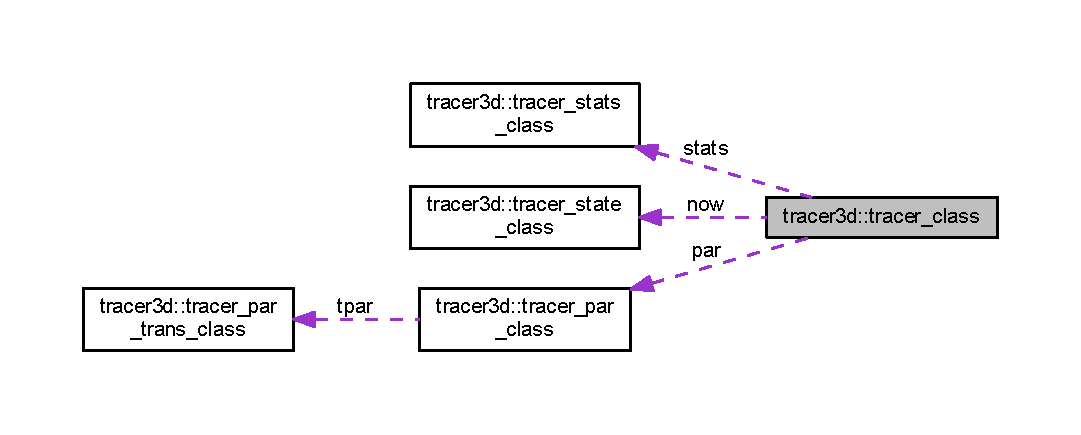
\includegraphics[width=350pt]{structtracer3d_1_1tracer__class__coll__graph}
\end{center}
\end{figure}
\subsection*{Private Attributes}
\begin{DoxyCompactItemize}
\item 
type(\mbox{\hyperlink{structtracer3d_1_1tracer__par__class}{tracer\+\_\+par\+\_\+class}}) \mbox{\hyperlink{structtracer3d_1_1tracer__class_a3745c68bd31158518852af7839b5d25d}{par}}
\begin{DoxyCompactList}\small\item\em To access parameters. \end{DoxyCompactList}\item 
type(\mbox{\hyperlink{structtracer3d_1_1tracer__state__class}{tracer\+\_\+state\+\_\+class}}) \mbox{\hyperlink{structtracer3d_1_1tracer__class_a9078a3dd8dfd7a789277f35549d31ff6}{now}}
\begin{DoxyCompactList}\small\item\em To access state variables. \end{DoxyCompactList}\item 
type(\mbox{\hyperlink{structtracer3d_1_1tracer__stats__class}{tracer\+\_\+stats\+\_\+class}}) \mbox{\hyperlink{structtracer3d_1_1tracer__class_a7145b520dad5b862da8b0fc14da0a8f0}{stats}}
\begin{DoxyCompactList}\small\item\em To access statistics. \end{DoxyCompactList}\end{DoxyCompactItemize}


\subsection{Detailed Description}
Type -\/ The pure Lagrangian tracer class. 

\subsection{Member Data Documentation}
\mbox{\Hypertarget{structtracer3d_1_1tracer__class_a9078a3dd8dfd7a789277f35549d31ff6}\label{structtracer3d_1_1tracer__class_a9078a3dd8dfd7a789277f35549d31ff6}} 
\index{tracer3d\+::tracer\+\_\+class@{tracer3d\+::tracer\+\_\+class}!now@{now}}
\index{now@{now}!tracer3d\+::tracer\+\_\+class@{tracer3d\+::tracer\+\_\+class}}
\subsubsection{\texorpdfstring{now}{now}}
{\footnotesize\ttfamily type(\mbox{\hyperlink{structtracer3d_1_1tracer__state__class}{tracer\+\_\+state\+\_\+class}}) tracer3d\+::tracer\+\_\+class\+::now\hspace{0.3cm}{\ttfamily [private]}}



To access state variables. 

\mbox{\Hypertarget{structtracer3d_1_1tracer__class_a3745c68bd31158518852af7839b5d25d}\label{structtracer3d_1_1tracer__class_a3745c68bd31158518852af7839b5d25d}} 
\index{tracer3d\+::tracer\+\_\+class@{tracer3d\+::tracer\+\_\+class}!par@{par}}
\index{par@{par}!tracer3d\+::tracer\+\_\+class@{tracer3d\+::tracer\+\_\+class}}
\subsubsection{\texorpdfstring{par}{par}}
{\footnotesize\ttfamily type(\mbox{\hyperlink{structtracer3d_1_1tracer__par__class}{tracer\+\_\+par\+\_\+class}}) tracer3d\+::tracer\+\_\+class\+::par\hspace{0.3cm}{\ttfamily [private]}}



To access parameters. 

\mbox{\Hypertarget{structtracer3d_1_1tracer__class_a7145b520dad5b862da8b0fc14da0a8f0}\label{structtracer3d_1_1tracer__class_a7145b520dad5b862da8b0fc14da0a8f0}} 
\index{tracer3d\+::tracer\+\_\+class@{tracer3d\+::tracer\+\_\+class}!stats@{stats}}
\index{stats@{stats}!tracer3d\+::tracer\+\_\+class@{tracer3d\+::tracer\+\_\+class}}
\subsubsection{\texorpdfstring{stats}{stats}}
{\footnotesize\ttfamily type(\mbox{\hyperlink{structtracer3d_1_1tracer__stats__class}{tracer\+\_\+stats\+\_\+class}}) tracer3d\+::tracer\+\_\+class\+::stats\hspace{0.3cm}{\ttfamily [private]}}



To access statistics. 



The documentation for this type was generated from the following file\+:\begin{DoxyCompactItemize}
\item 
C\+:/\+Users/administrator/\+Documents/\+Git\+Hub/\+M\+O\+H\+I\+D-\/\+Lagrangian/src/lib/\mbox{\hyperlink{tracer3_d_8f90}{tracer3\+D.\+f90}}\end{DoxyCompactItemize}

\hypertarget{structtracer3d_1_1tracer__dep__class}{}\section{tracer3d\+:\+:tracer\+\_\+dep\+\_\+class Type Reference}
\label{structtracer3d_1_1tracer__dep__class}\index{tracer3d\+::tracer\+\_\+dep\+\_\+class@{tracer3d\+::tracer\+\_\+dep\+\_\+class}}
\subsection*{Public Attributes}
\begin{DoxyCompactItemize}
\item 
\mbox{\Hypertarget{structtracer3d_1_1tracer__dep__class_a0ff57f50a335e245c2a7b37b4b6f27b5}\label{structtracer3d_1_1tracer__dep__class_a0ff57f50a335e245c2a7b37b4b6f27b5}} 
real(prec), dimension(\+:), allocatable {\bfseries time}
\item 
\mbox{\Hypertarget{structtracer3d_1_1tracer__dep__class_a717aeb47146fd7af90eb4a19a36f925d}\label{structtracer3d_1_1tracer__dep__class_a717aeb47146fd7af90eb4a19a36f925d}} 
real(prec), dimension(\+:), allocatable {\bfseries h}
\item 
\mbox{\Hypertarget{structtracer3d_1_1tracer__dep__class_ad8c69db37dfd9db720c53bb6764842c5}\label{structtracer3d_1_1tracer__dep__class_ad8c69db37dfd9db720c53bb6764842c5}} 
real(prec), dimension(\+:), allocatable {\bfseries x}
\item 
\mbox{\Hypertarget{structtracer3d_1_1tracer__dep__class_a414a5a1630400d24ae0e53444b1ce6b2}\label{structtracer3d_1_1tracer__dep__class_a414a5a1630400d24ae0e53444b1ce6b2}} 
real(prec), dimension(\+:), allocatable {\bfseries y}
\item 
\mbox{\Hypertarget{structtracer3d_1_1tracer__dep__class_ab7fc71bff2efc5ffcbfbe1e6e118e270}\label{structtracer3d_1_1tracer__dep__class_ab7fc71bff2efc5ffcbfbe1e6e118e270}} 
real(prec), dimension(\+:), allocatable {\bfseries z}
\item 
\mbox{\Hypertarget{structtracer3d_1_1tracer__dep__class_aa4961c950509149eae12e72882da7b97}\label{structtracer3d_1_1tracer__dep__class_aa4961c950509149eae12e72882da7b97}} 
real(prec), dimension(\+:), allocatable {\bfseries lon}
\item 
\mbox{\Hypertarget{structtracer3d_1_1tracer__dep__class_a6b2d5c6a9bc8e11b0237fca79a21c62e}\label{structtracer3d_1_1tracer__dep__class_a6b2d5c6a9bc8e11b0237fca79a21c62e}} 
real(prec), dimension(\+:), allocatable {\bfseries lat}
\item 
\mbox{\Hypertarget{structtracer3d_1_1tracer__dep__class_a4345f4c12352a0a61170b9ae6253cb3d}\label{structtracer3d_1_1tracer__dep__class_a4345f4c12352a0a61170b9ae6253cb3d}} 
real(prec), dimension(\+:), allocatable {\bfseries t2m\+\_\+ann}
\item 
\mbox{\Hypertarget{structtracer3d_1_1tracer__dep__class_a4d752a062b60d3ca6bb48fc3b396a4ad}\label{structtracer3d_1_1tracer__dep__class_a4d752a062b60d3ca6bb48fc3b396a4ad}} 
real(prec), dimension(\+:), allocatable {\bfseries t2m\+\_\+sum}
\item 
\mbox{\Hypertarget{structtracer3d_1_1tracer__dep__class_a95132f8073ed9606a3d970add2d64acd}\label{structtracer3d_1_1tracer__dep__class_a95132f8073ed9606a3d970add2d64acd}} 
real(prec), dimension(\+:), allocatable {\bfseries pr\+\_\+ann}
\item 
\mbox{\Hypertarget{structtracer3d_1_1tracer__dep__class_abe74cc6e8d31ea0ba3d00351b4c8b8db}\label{structtracer3d_1_1tracer__dep__class_abe74cc6e8d31ea0ba3d00351b4c8b8db}} 
real(prec), dimension(\+:), allocatable {\bfseries pr\+\_\+sum}
\item 
\mbox{\Hypertarget{structtracer3d_1_1tracer__dep__class_abb18f335dbe324d663ef696d47409316}\label{structtracer3d_1_1tracer__dep__class_abb18f335dbe324d663ef696d47409316}} 
real(prec), dimension(\+:), allocatable {\bfseries t2m\+\_\+prann}
\item 
\mbox{\Hypertarget{structtracer3d_1_1tracer__dep__class_ad1d5702c4c242bf9d15618d6c34835d2}\label{structtracer3d_1_1tracer__dep__class_ad1d5702c4c242bf9d15618d6c34835d2}} 
real(prec), dimension(\+:), allocatable {\bfseries d18o\+\_\+ann}
\end{DoxyCompactItemize}


The documentation for this type was generated from the following file\+:\begin{DoxyCompactItemize}
\item 
src/lib/tracer3\+D.\+f90\end{DoxyCompactItemize}

\hypertarget{structtracer3d_1_1tracer__par__class}{}\section{tracer3d\+:\+:tracer\+\_\+par\+\_\+class Type Reference}
\label{structtracer3d_1_1tracer__par__class}\index{tracer3d\+::tracer\+\_\+par\+\_\+class@{tracer3d\+::tracer\+\_\+par\+\_\+class}}
\subsection*{Public Attributes}
\begin{DoxyCompactItemize}
\item 
\mbox{\Hypertarget{structtracer3d_1_1tracer__par__class_afee9b223da2104cc94d7925a09ce1b5b}\label{structtracer3d_1_1tracer__par__class_afee9b223da2104cc94d7925a09ce1b5b}} 
integer \mbox{\hyperlink{structtracer3d_1_1tracer__par__class_afee9b223da2104cc94d7925a09ce1b5b}{n}}
\begin{DoxyCompactList}\small\item\em Type -\/ parameters of a pure Lagrangian tracer object. \end{DoxyCompactList}\item 
\mbox{\Hypertarget{structtracer3d_1_1tracer__par__class_a595e743676b4b97d7b6895ce1da701c2}\label{structtracer3d_1_1tracer__par__class_a595e743676b4b97d7b6895ce1da701c2}} 
integer {\bfseries n\+\_\+active}
\item 
\mbox{\Hypertarget{structtracer3d_1_1tracer__par__class_a88718350ee32f1a882264dd68ed377a8}\label{structtracer3d_1_1tracer__par__class_a88718350ee32f1a882264dd68ed377a8}} 
integer {\bfseries n\+\_\+max\+\_\+dep}
\item 
\mbox{\Hypertarget{structtracer3d_1_1tracer__par__class_a249769f71ff720d3ac6d594c7670f507}\label{structtracer3d_1_1tracer__par__class_a249769f71ff720d3ac6d594c7670f507}} 
integer {\bfseries id\+\_\+max}
\item 
\mbox{\Hypertarget{structtracer3d_1_1tracer__par__class_ab3070eb172aec777973175d521fde0d4}\label{structtracer3d_1_1tracer__par__class_ab3070eb172aec777973175d521fde0d4}} 
logical {\bfseries is\+\_\+sigma}
\item 
\mbox{\Hypertarget{structtracer3d_1_1tracer__par__class_a17d4f4f2e5c564cfd71aec5a9c86e9ae}\label{structtracer3d_1_1tracer__par__class_a17d4f4f2e5c564cfd71aec5a9c86e9ae}} 
real(prec\+\_\+time) {\bfseries dt}
\item 
\mbox{\Hypertarget{structtracer3d_1_1tracer__par__class_a03f19bcc6a1d85314b1e79b3339092fa}\label{structtracer3d_1_1tracer__par__class_a03f19bcc6a1d85314b1e79b3339092fa}} 
real(prec\+\_\+time) {\bfseries dt\+\_\+dep}
\item 
\mbox{\Hypertarget{structtracer3d_1_1tracer__par__class_a3c25026d05e257ab283072e7c112311b}\label{structtracer3d_1_1tracer__par__class_a3c25026d05e257ab283072e7c112311b}} 
real(prec\+\_\+time) {\bfseries dt\+\_\+write}
\item 
\mbox{\Hypertarget{structtracer3d_1_1tracer__par__class_acf2b12b8eaf5570a8f0ba0d12222269f}\label{structtracer3d_1_1tracer__par__class_acf2b12b8eaf5570a8f0ba0d12222269f}} 
real(prec) {\bfseries thk\+\_\+min}
\item 
\mbox{\Hypertarget{structtracer3d_1_1tracer__par__class_a475d343b54e274b8dfe70268f95c4d3f}\label{structtracer3d_1_1tracer__par__class_a475d343b54e274b8dfe70268f95c4d3f}} 
real(prec) {\bfseries h\+\_\+min}
\item 
\mbox{\Hypertarget{structtracer3d_1_1tracer__par__class_afff0b95b0ab6d6aad07f2bd25f74b9dc}\label{structtracer3d_1_1tracer__par__class_afff0b95b0ab6d6aad07f2bd25f74b9dc}} 
real(prec) {\bfseries depth\+\_\+max}
\item 
\mbox{\Hypertarget{structtracer3d_1_1tracer__par__class_ad0ae3a7d44261e8f378184ced0b61972}\label{structtracer3d_1_1tracer__par__class_ad0ae3a7d44261e8f378184ced0b61972}} 
real(prec) {\bfseries u\+\_\+max}
\item 
\mbox{\Hypertarget{structtracer3d_1_1tracer__par__class_a5d490688e99c3590ca3615f61da57d78}\label{structtracer3d_1_1tracer__par__class_a5d490688e99c3590ca3615f61da57d78}} 
real(prec) {\bfseries u\+\_\+max\+\_\+dep}
\item 
\mbox{\Hypertarget{structtracer3d_1_1tracer__par__class_a18eff67cc1119b68f8301a1aa78da899}\label{structtracer3d_1_1tracer__par__class_a18eff67cc1119b68f8301a1aa78da899}} 
real(prec) {\bfseries h\+\_\+min\+\_\+dep}
\item 
\mbox{\Hypertarget{structtracer3d_1_1tracer__par__class_a7784a45b39d84e70b44df3afda935acb}\label{structtracer3d_1_1tracer__par__class_a7784a45b39d84e70b44df3afda935acb}} 
real(prec) {\bfseries alpha}
\item 
\mbox{\Hypertarget{structtracer3d_1_1tracer__par__class_a4414deb31b8791b1cdf5ca5646d14225}\label{structtracer3d_1_1tracer__par__class_a4414deb31b8791b1cdf5ca5646d14225}} 
character(len=56) {\bfseries weight}
\item 
\mbox{\Hypertarget{structtracer3d_1_1tracer__par__class_af258b7ca349ce911511dbd89b24606f7}\label{structtracer3d_1_1tracer__par__class_af258b7ca349ce911511dbd89b24606f7}} 
logical {\bfseries noise}
\item 
\mbox{\Hypertarget{structtracer3d_1_1tracer__par__class_aadbc554683f144875a2a0dd60baa5450}\label{structtracer3d_1_1tracer__par__class_aadbc554683f144875a2a0dd60baa5450}} 
real(prec) {\bfseries dens\+\_\+z\+\_\+lim}
\item 
\mbox{\Hypertarget{structtracer3d_1_1tracer__par__class_a7617f9085e28d93250ebed7ad6007869}\label{structtracer3d_1_1tracer__par__class_a7617f9085e28d93250ebed7ad6007869}} 
integer {\bfseries dens\+\_\+max}
\item 
\mbox{\Hypertarget{structtracer3d_1_1tracer__par__class_a33c8edd729f2f4c19571ee04368be4e0}\label{structtracer3d_1_1tracer__par__class_a33c8edd729f2f4c19571ee04368be4e0}} 
character(len=56) {\bfseries interp\+\_\+method}
\item 
\mbox{\Hypertarget{structtracer3d_1_1tracer__par__class_a502b51714ceeed6e028b0eaea8fc41b4}\label{structtracer3d_1_1tracer__par__class_a502b51714ceeed6e028b0eaea8fc41b4}} 
character(len=512) {\bfseries par\+\_\+trans\+\_\+file}
\item 
\mbox{\Hypertarget{structtracer3d_1_1tracer__par__class_a9bb9fd6b9779087e2db2805a803ac736}\label{structtracer3d_1_1tracer__par__class_a9bb9fd6b9779087e2db2805a803ac736}} 
logical {\bfseries use\+\_\+par\+\_\+trans}
\item 
\mbox{\Hypertarget{structtracer3d_1_1tracer__par__class_a4486f0959101435f0fdeb1c845d4bbf4}\label{structtracer3d_1_1tracer__par__class_a4486f0959101435f0fdeb1c845d4bbf4}} 
type(\mbox{\hyperlink{structtracer3d_1_1tracer__par__trans__class}{tracer\+\_\+par\+\_\+trans\+\_\+class}}) {\bfseries tpar}
\end{DoxyCompactItemize}


The documentation for this type was generated from the following file\+:\begin{DoxyCompactItemize}
\item 
src/lib/tracer3\+D.\+f90\end{DoxyCompactItemize}

\hypertarget{structtracer3d_1_1tracer__par__trans__class}{}\section{tracer3d\+:\+:tracer\+\_\+par\+\_\+trans\+\_\+class Type Reference}
\label{structtracer3d_1_1tracer__par__trans__class}\index{tracer3d\+::tracer\+\_\+par\+\_\+trans\+\_\+class@{tracer3d\+::tracer\+\_\+par\+\_\+trans\+\_\+class}}
\subsection*{Public Attributes}
\begin{DoxyCompactItemize}
\item 
\mbox{\Hypertarget{structtracer3d_1_1tracer__par__trans__class_acd1f347b090a9d50fb5c248bfd5382e4}\label{structtracer3d_1_1tracer__par__trans__class_acd1f347b090a9d50fb5c248bfd5382e4}} 
integer \mbox{\hyperlink{structtracer3d_1_1tracer__par__trans__class_acd1f347b090a9d50fb5c248bfd5382e4}{nt}}
\begin{DoxyCompactList}\small\item\em Type -\/ transient parameters of a pure Lagrangian tracer object. \end{DoxyCompactList}\item 
\mbox{\Hypertarget{structtracer3d_1_1tracer__par__trans__class_acf9adabf777d904bd8b763cfeb8a4e94}\label{structtracer3d_1_1tracer__par__trans__class_acf9adabf777d904bd8b763cfeb8a4e94}} 
real(prec), dimension(\+:), allocatable {\bfseries time}
\item 
\mbox{\Hypertarget{structtracer3d_1_1tracer__par__trans__class_a62efb8dbf563d10983dfdf951d2628dc}\label{structtracer3d_1_1tracer__par__trans__class_a62efb8dbf563d10983dfdf951d2628dc}} 
real(prec), dimension(\+:), allocatable {\bfseries h\+\_\+min\+\_\+dep}
\item 
\mbox{\Hypertarget{structtracer3d_1_1tracer__par__trans__class_a076f420209f6c2ff1aa118c93c7d1506}\label{structtracer3d_1_1tracer__par__trans__class_a076f420209f6c2ff1aa118c93c7d1506}} 
real(prec), dimension(\+:), allocatable {\bfseries dt\+\_\+dep}
\item 
\mbox{\Hypertarget{structtracer3d_1_1tracer__par__trans__class_ac5403415223ceab61201747c6d141f51}\label{structtracer3d_1_1tracer__par__trans__class_ac5403415223ceab61201747c6d141f51}} 
integer, dimension(\+:), allocatable {\bfseries n\+\_\+max\+\_\+dep}
\item 
\mbox{\Hypertarget{structtracer3d_1_1tracer__par__trans__class_abd94365b132aef667b12859310a6fb3c}\label{structtracer3d_1_1tracer__par__trans__class_abd94365b132aef667b12859310a6fb3c}} 
real(prec), dimension(\+:), allocatable {\bfseries dt\+\_\+write}
\end{DoxyCompactItemize}


The documentation for this type was generated from the following file\+:\begin{DoxyCompactItemize}
\item 
src/lib/tracer3\+D.\+f90\end{DoxyCompactItemize}

\hypertarget{structtracer3d_1_1tracer__state__class}{}\section{tracer3d\+:\+:tracer\+\_\+state\+\_\+class Type Reference}
\label{structtracer3d_1_1tracer__state__class}\index{tracer3d\+::tracer\+\_\+state\+\_\+class@{tracer3d\+::tracer\+\_\+state\+\_\+class}}
\subsection*{Public Attributes}
\begin{DoxyCompactItemize}
\item 
\mbox{\Hypertarget{structtracer3d_1_1tracer__state__class_ad2c406b0c70535b9eefc6a58b5155228}\label{structtracer3d_1_1tracer__state__class_ad2c406b0c70535b9eefc6a58b5155228}} 
real(prec\+\_\+time) \mbox{\hyperlink{structtracer3d_1_1tracer__state__class_ad2c406b0c70535b9eefc6a58b5155228}{time}}
\begin{DoxyCompactList}\small\item\em Type -\/ state variables of a pure Lagrangian tracer object. \end{DoxyCompactList}\item 
\mbox{\Hypertarget{structtracer3d_1_1tracer__state__class_aff3f9a1333320499aae96ab6e0d31ded}\label{structtracer3d_1_1tracer__state__class_aff3f9a1333320499aae96ab6e0d31ded}} 
real(prec\+\_\+time) {\bfseries time\+\_\+old}
\item 
\mbox{\Hypertarget{structtracer3d_1_1tracer__state__class_a45e7a5c8c9fb20695d004397ab2ceaee}\label{structtracer3d_1_1tracer__state__class_a45e7a5c8c9fb20695d004397ab2ceaee}} 
real(prec\+\_\+time) {\bfseries time\+\_\+dep}
\item 
\mbox{\Hypertarget{structtracer3d_1_1tracer__state__class_a4778a9a01005ff19c20dbba6c081c4b9}\label{structtracer3d_1_1tracer__state__class_a4778a9a01005ff19c20dbba6c081c4b9}} 
real(prec\+\_\+time) {\bfseries time\+\_\+write}
\item 
\mbox{\Hypertarget{structtracer3d_1_1tracer__state__class_aff1762f7b19fc4480e8ab2562ccbb9e6}\label{structtracer3d_1_1tracer__state__class_aff1762f7b19fc4480e8ab2562ccbb9e6}} 
real(prec\+\_\+time) {\bfseries dt}
\item 
\mbox{\Hypertarget{structtracer3d_1_1tracer__state__class_ab350c849df637157d07b05d6df6cd035}\label{structtracer3d_1_1tracer__state__class_ab350c849df637157d07b05d6df6cd035}} 
integer, dimension(\+:), allocatable {\bfseries active}
\item 
\mbox{\Hypertarget{structtracer3d_1_1tracer__state__class_a047e35293ddbc8f44235b95db1400cc6}\label{structtracer3d_1_1tracer__state__class_a047e35293ddbc8f44235b95db1400cc6}} 
integer, dimension(\+:), allocatable {\bfseries id}
\item 
\mbox{\Hypertarget{structtracer3d_1_1tracer__state__class_a3dd71636cabb59e0138620d91b936b78}\label{structtracer3d_1_1tracer__state__class_a3dd71636cabb59e0138620d91b936b78}} 
real(prec), dimension(\+:), allocatable {\bfseries x}
\item 
\mbox{\Hypertarget{structtracer3d_1_1tracer__state__class_af37256105de6c1965ad3ec817d1793c2}\label{structtracer3d_1_1tracer__state__class_af37256105de6c1965ad3ec817d1793c2}} 
real(prec), dimension(\+:), allocatable {\bfseries y}
\item 
\mbox{\Hypertarget{structtracer3d_1_1tracer__state__class_ae68109f8656e4a460ac598a09fcd7d91}\label{structtracer3d_1_1tracer__state__class_ae68109f8656e4a460ac598a09fcd7d91}} 
real(prec), dimension(\+:), allocatable {\bfseries z}
\item 
\mbox{\Hypertarget{structtracer3d_1_1tracer__state__class_a2327dc43d8a234c7898d7d6804eb9674}\label{structtracer3d_1_1tracer__state__class_a2327dc43d8a234c7898d7d6804eb9674}} 
real(prec), dimension(\+:), allocatable {\bfseries sigma}
\item 
\mbox{\Hypertarget{structtracer3d_1_1tracer__state__class_ab91de1a2ec3332cf6ab5f694fb6c7e8b}\label{structtracer3d_1_1tracer__state__class_ab91de1a2ec3332cf6ab5f694fb6c7e8b}} 
real(prec), dimension(\+:), allocatable {\bfseries ux}
\item 
\mbox{\Hypertarget{structtracer3d_1_1tracer__state__class_ae6822a2f1d48bd274351eef5257e3757}\label{structtracer3d_1_1tracer__state__class_ae6822a2f1d48bd274351eef5257e3757}} 
real(prec), dimension(\+:), allocatable {\bfseries uy}
\item 
\mbox{\Hypertarget{structtracer3d_1_1tracer__state__class_a8379b1be1b73a1ce6737fcd332cca3dc}\label{structtracer3d_1_1tracer__state__class_a8379b1be1b73a1ce6737fcd332cca3dc}} 
real(prec), dimension(\+:), allocatable {\bfseries uz}
\item 
\mbox{\Hypertarget{structtracer3d_1_1tracer__state__class_a82dbab042574c76501610500805392c2}\label{structtracer3d_1_1tracer__state__class_a82dbab042574c76501610500805392c2}} 
real(prec), dimension(\+:), allocatable {\bfseries ax}
\item 
\mbox{\Hypertarget{structtracer3d_1_1tracer__state__class_add9d471862791f397e2788e4e14b345b}\label{structtracer3d_1_1tracer__state__class_add9d471862791f397e2788e4e14b345b}} 
real(prec), dimension(\+:), allocatable {\bfseries ay}
\item 
\mbox{\Hypertarget{structtracer3d_1_1tracer__state__class_afbe58ebc71d95db831507b307d28a5b6}\label{structtracer3d_1_1tracer__state__class_afbe58ebc71d95db831507b307d28a5b6}} 
real(prec), dimension(\+:), allocatable {\bfseries az}
\item 
\mbox{\Hypertarget{structtracer3d_1_1tracer__state__class_a1b967658f4f0a5c0d727b02be993e241}\label{structtracer3d_1_1tracer__state__class_a1b967658f4f0a5c0d727b02be993e241}} 
real(prec), dimension(\+:), allocatable {\bfseries dpth}
\item 
\mbox{\Hypertarget{structtracer3d_1_1tracer__state__class_ae5dd01566aa84508017ea302356a263b}\label{structtracer3d_1_1tracer__state__class_ae5dd01566aa84508017ea302356a263b}} 
real(prec), dimension(\+:), allocatable {\bfseries z\+\_\+srf}
\item 
\mbox{\Hypertarget{structtracer3d_1_1tracer__state__class_aba3e3096026a8e8f090c2580944fd681}\label{structtracer3d_1_1tracer__state__class_aba3e3096026a8e8f090c2580944fd681}} 
real(prec), dimension(\+:), allocatable {\bfseries thk}
\item 
\mbox{\Hypertarget{structtracer3d_1_1tracer__state__class_ae64e9e0c66c93ee01bf9fa9049c9a381}\label{structtracer3d_1_1tracer__state__class_ae64e9e0c66c93ee01bf9fa9049c9a381}} 
real(prec), dimension(\+:), allocatable {\bfseries t}
\item 
\mbox{\Hypertarget{structtracer3d_1_1tracer__state__class_a8b97bd7e1174f0b475186c6784b0d5ec}\label{structtracer3d_1_1tracer__state__class_a8b97bd7e1174f0b475186c6784b0d5ec}} 
real(prec), dimension(\+:), allocatable {\bfseries h}
\end{DoxyCompactItemize}


The documentation for this type was generated from the following file\+:\begin{DoxyCompactItemize}
\item 
src/lib/tracer3\+D.\+f90\end{DoxyCompactItemize}

\hypertarget{structtracer3d_1_1tracer__stats__class}{}\section{tracer3d\+:\+:tracer\+\_\+stats\+\_\+class Type Reference}
\label{structtracer3d_1_1tracer__stats__class}\index{tracer3d\+::tracer\+\_\+stats\+\_\+class@{tracer3d\+::tracer\+\_\+stats\+\_\+class}}


Type -\/ statistical variables of a pure Lagrangian tracer object.  


\subsection*{Private Attributes}
\begin{DoxyCompactItemize}
\item 
type(vector) \mbox{\hyperlink{structtracer3d_1_1tracer__stats__class_a1a9df2788c632bb2dcba4e303dc83e78}{acc\+\_\+pos}}
\begin{DoxyCompactList}\small\item\em Accumulated position of the tracer (m) \end{DoxyCompactList}\item 
type(vector) \mbox{\hyperlink{structtracer3d_1_1tracer__stats__class_a623f27a49b6e37a3e5c21b8bab55a323}{acc\+\_\+vel}}
\begin{DoxyCompactList}\small\item\em Accumulated velocity of the tracer (m s-\/1) \end{DoxyCompactList}\item 
real(prec\+\_\+wrt) \mbox{\hyperlink{structtracer3d_1_1tracer__stats__class_af9e6304d89967e9ade6b1188101391b6}{acc\+\_\+depth}}
\begin{DoxyCompactList}\small\item\em Accumulated depth of the tracer (m) \end{DoxyCompactList}\item 
real(prec\+\_\+wrt) \mbox{\hyperlink{structtracer3d_1_1tracer__stats__class_acdca78550575d7690eb26482ed75aeef}{acc\+\_\+t}}
\begin{DoxyCompactList}\small\item\em Accumulated temperature of the tracer (Celcius) \end{DoxyCompactList}\item 
integer \mbox{\hyperlink{structtracer3d_1_1tracer__stats__class_a0a07132ada5734cd6f132bc9ffd327b2}{ns}}
\begin{DoxyCompactList}\small\item\em Number of sampling steps. \end{DoxyCompactList}\end{DoxyCompactItemize}


\subsection{Detailed Description}
Type -\/ statistical variables of a pure Lagrangian tracer object. 

\subsection{Member Data Documentation}
\mbox{\Hypertarget{structtracer3d_1_1tracer__stats__class_af9e6304d89967e9ade6b1188101391b6}\label{structtracer3d_1_1tracer__stats__class_af9e6304d89967e9ade6b1188101391b6}} 
\index{tracer3d\+::tracer\+\_\+stats\+\_\+class@{tracer3d\+::tracer\+\_\+stats\+\_\+class}!acc\+\_\+depth@{acc\+\_\+depth}}
\index{acc\+\_\+depth@{acc\+\_\+depth}!tracer3d\+::tracer\+\_\+stats\+\_\+class@{tracer3d\+::tracer\+\_\+stats\+\_\+class}}
\subsubsection{\texorpdfstring{acc\+\_\+depth}{acc\_depth}}
{\footnotesize\ttfamily real(prec\+\_\+wrt) tracer3d\+::tracer\+\_\+stats\+\_\+class\+::acc\+\_\+depth\hspace{0.3cm}{\ttfamily [private]}}



Accumulated depth of the tracer (m) 

\mbox{\Hypertarget{structtracer3d_1_1tracer__stats__class_a1a9df2788c632bb2dcba4e303dc83e78}\label{structtracer3d_1_1tracer__stats__class_a1a9df2788c632bb2dcba4e303dc83e78}} 
\index{tracer3d\+::tracer\+\_\+stats\+\_\+class@{tracer3d\+::tracer\+\_\+stats\+\_\+class}!acc\+\_\+pos@{acc\+\_\+pos}}
\index{acc\+\_\+pos@{acc\+\_\+pos}!tracer3d\+::tracer\+\_\+stats\+\_\+class@{tracer3d\+::tracer\+\_\+stats\+\_\+class}}
\subsubsection{\texorpdfstring{acc\+\_\+pos}{acc\_pos}}
{\footnotesize\ttfamily type(vector) tracer3d\+::tracer\+\_\+stats\+\_\+class\+::acc\+\_\+pos\hspace{0.3cm}{\ttfamily [private]}}



Accumulated position of the tracer (m) 

\mbox{\Hypertarget{structtracer3d_1_1tracer__stats__class_acdca78550575d7690eb26482ed75aeef}\label{structtracer3d_1_1tracer__stats__class_acdca78550575d7690eb26482ed75aeef}} 
\index{tracer3d\+::tracer\+\_\+stats\+\_\+class@{tracer3d\+::tracer\+\_\+stats\+\_\+class}!acc\+\_\+t@{acc\+\_\+t}}
\index{acc\+\_\+t@{acc\+\_\+t}!tracer3d\+::tracer\+\_\+stats\+\_\+class@{tracer3d\+::tracer\+\_\+stats\+\_\+class}}
\subsubsection{\texorpdfstring{acc\+\_\+t}{acc\_t}}
{\footnotesize\ttfamily real(prec\+\_\+wrt) tracer3d\+::tracer\+\_\+stats\+\_\+class\+::acc\+\_\+t\hspace{0.3cm}{\ttfamily [private]}}



Accumulated temperature of the tracer (Celcius) 

\mbox{\Hypertarget{structtracer3d_1_1tracer__stats__class_a623f27a49b6e37a3e5c21b8bab55a323}\label{structtracer3d_1_1tracer__stats__class_a623f27a49b6e37a3e5c21b8bab55a323}} 
\index{tracer3d\+::tracer\+\_\+stats\+\_\+class@{tracer3d\+::tracer\+\_\+stats\+\_\+class}!acc\+\_\+vel@{acc\+\_\+vel}}
\index{acc\+\_\+vel@{acc\+\_\+vel}!tracer3d\+::tracer\+\_\+stats\+\_\+class@{tracer3d\+::tracer\+\_\+stats\+\_\+class}}
\subsubsection{\texorpdfstring{acc\+\_\+vel}{acc\_vel}}
{\footnotesize\ttfamily type(vector) tracer3d\+::tracer\+\_\+stats\+\_\+class\+::acc\+\_\+vel\hspace{0.3cm}{\ttfamily [private]}}



Accumulated velocity of the tracer (m s-\/1) 

\mbox{\Hypertarget{structtracer3d_1_1tracer__stats__class_a0a07132ada5734cd6f132bc9ffd327b2}\label{structtracer3d_1_1tracer__stats__class_a0a07132ada5734cd6f132bc9ffd327b2}} 
\index{tracer3d\+::tracer\+\_\+stats\+\_\+class@{tracer3d\+::tracer\+\_\+stats\+\_\+class}!ns@{ns}}
\index{ns@{ns}!tracer3d\+::tracer\+\_\+stats\+\_\+class@{tracer3d\+::tracer\+\_\+stats\+\_\+class}}
\subsubsection{\texorpdfstring{ns}{ns}}
{\footnotesize\ttfamily integer tracer3d\+::tracer\+\_\+stats\+\_\+class\+::ns\hspace{0.3cm}{\ttfamily [private]}}



Number of sampling steps. 



The documentation for this type was generated from the following file\+:\begin{DoxyCompactItemize}
\item 
C\+:/\+Users/administrator/\+Documents/\+Git\+Hub/\+M\+O\+H\+I\+D-\/\+Lagrangian/src/lib/\mbox{\hyperlink{tracer3_d_8f90}{tracer3\+D.\+f90}}\end{DoxyCompactItemize}

%--- End generated contents ---

% Index
\backmatter
\newpage
\phantomsection
\clearemptydoublepage
\addcontentsline{toc}{chapter}{Index}
\printindex

\end{document}
